\chapter{Výsledky práce}
Vytvorili sme budík na platforme Arduino Uno s využitím modulu reálneho času a LCD displeja. Implementované riešenie spĺňa všetky požiadavky kladené v cieľoch práce a demonštuje nektoré možnosti zvolenej platformy.

Snažili sme sa tiež navrhnúť dostatočne jednoduché a intuitívne ovládanie vzhľadom na možnosti poskytnuté použitými komponentmi. Pre úplnosť je návod na použitie uvedený v nasledujúcej sekcii.

\section{Ovládanie}
V základnom režime budík zobrazuje dátum, čas a teplotu. Pri neaktivite sa stlmí podsvietenie displeja.

\begin{figure}[h]
    \centering
    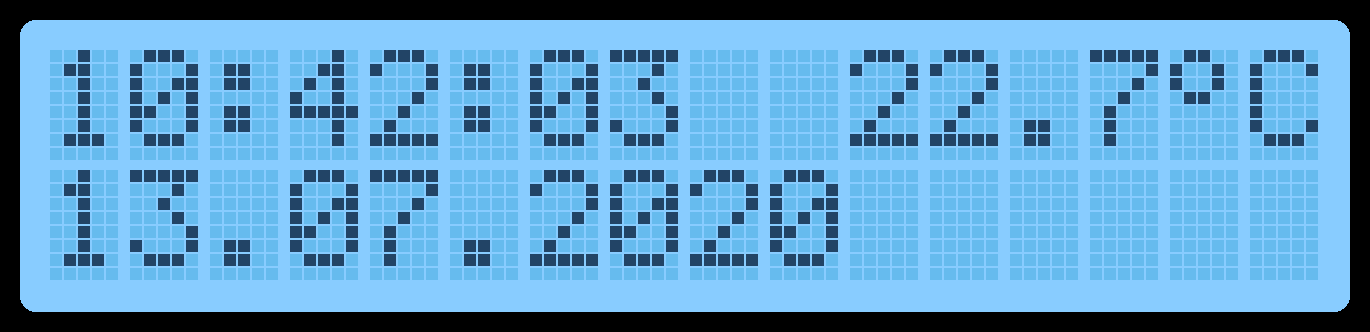
\includegraphics[width=0.7\textwidth]{img/display_time.png}
    \caption{Zobrazenie dátumu, času a teploty v základnom režime.}
\end{figure}

Pre nastavenie času budenia stlačíme tlačidlo \texttt{A}. Následne je možné tlačidlami zadať požadovaý čas budenia a potvrdiť tlačidlom \texttt{\#}.

\begin{figure}[h]
    \centering
    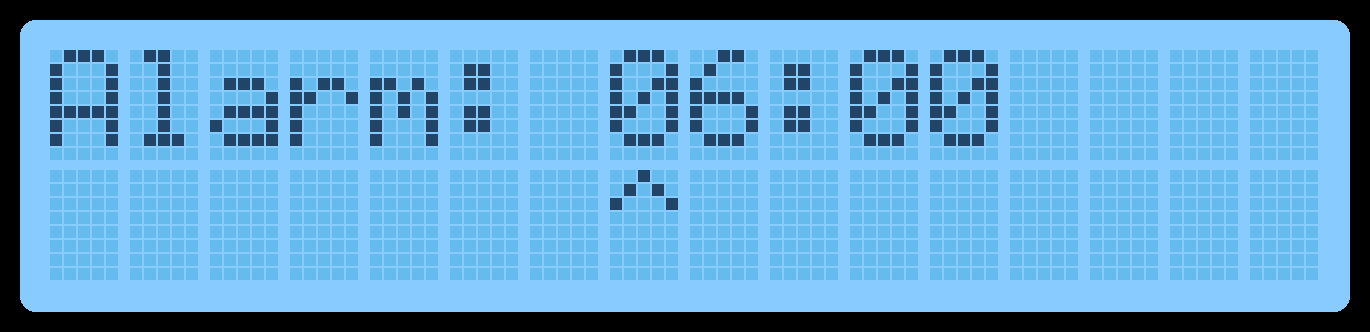
\includegraphics[width=0.7\textwidth]{img/display_set_alarm.png}
    \caption{Nastavenie času budenia.}
\end{figure}

Vo zvolenom čase budík začne budiť hlasným tónom a na displeji sa zobrazí výzva na zadanie hesla. Heslo je možné zadať tlačidlami a potvrdiť tlačidlom \texttt{\#}. Ak je heslo správne, budík sa stíši, v opačnom prípade bude zvoniť ďalej.

\begin{figure}[h]
    \centering
    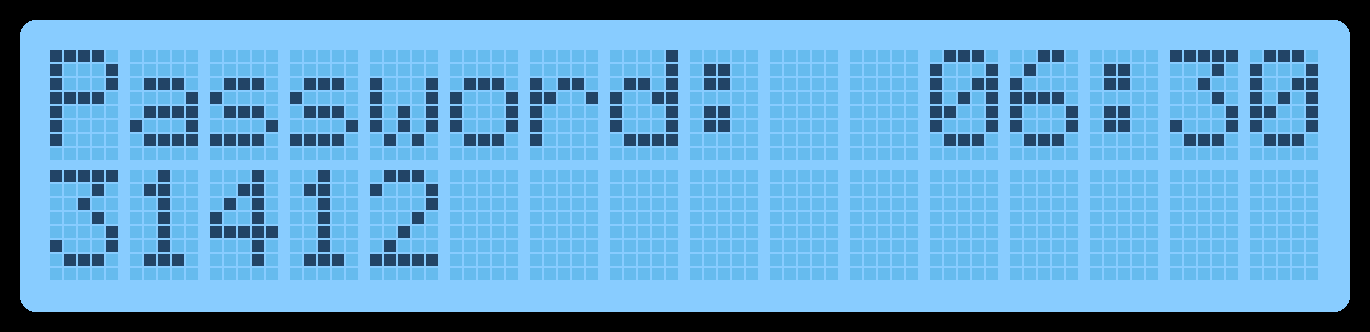
\includegraphics[width=0.7\textwidth]{img/display_alarm.png}
    \caption{Budenie.}
\end{figure}

Pre nastavenie vlastného hesla stlačíme tlačidlo \texttt{B}. Následne je možné tlačidlami zadať nové heslo a potvrdiť tlačidlom \texttt{\#}.

\begin{figure}[h]
    \centering
    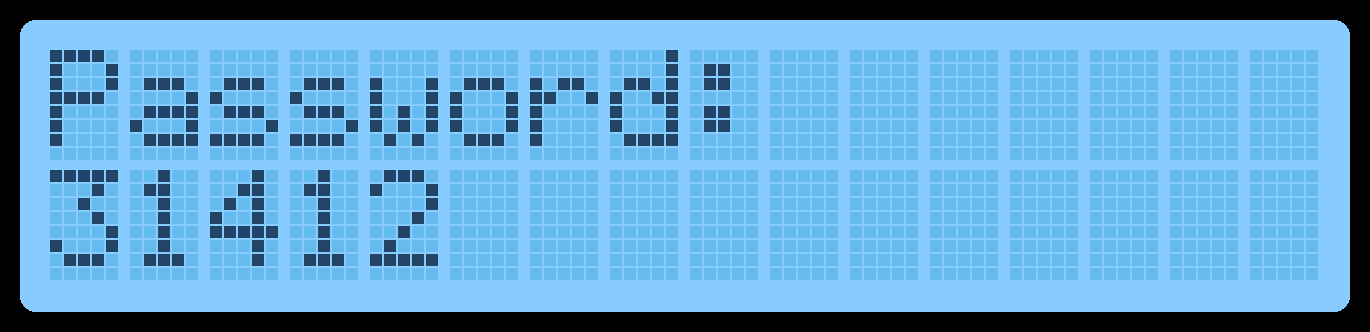
\includegraphics[width=0.7\textwidth]{img/display_set_pass.png}
    \caption{Nastavenie hesla.}
\end{figure}
